\chapter{MDI and the G-code Editor}
\label{ch:mdi}

\section{MDI: one block at a time}

MDI is a working area, not a text box. Turn the selector to \textbf{MDI} and the Machine page
opens with the MDI pane in the slot the program card normally fills.

\begin{figure}[H]
  \centering
  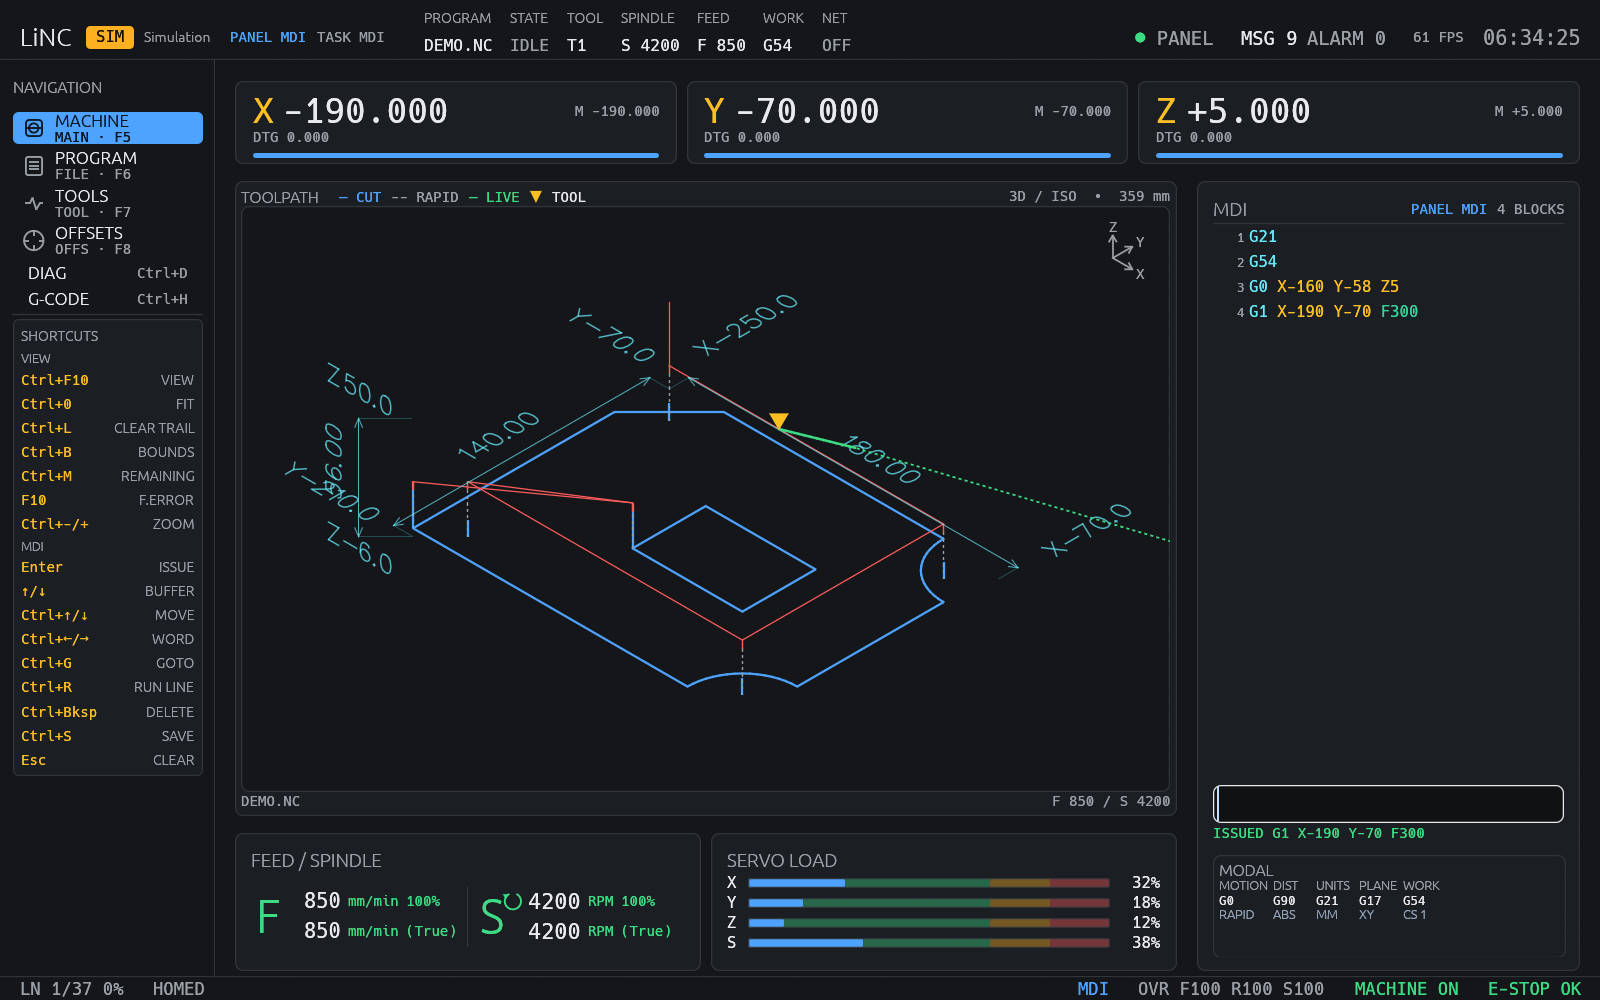
\includegraphics[width=\textwidth]{img/ui/mdi.png}
  \caption{The MDI pane on the Machine page: the blocks already issued, the input line, the
           result strip, the modal band, and the block being typed drawn on the toolpath.}
  \label{fig:mdi}
\end{figure}

The pane, top to bottom:

\begin{itemize}
  \item \textbf{The buffer}: every block issued in this session, in order, with a selection
        band on the row the arrow keys point at.
  \item \textbf{The input}: one syntax-highlighted line. It holds the keyboard by default, so
        a block can be typed as soon as the pane appears.
  \item \textbf{The result strip}: the last issue result, or the validation error that stopped
        it.
  \item \textbf{The modal band}: the same active codes the AUTO program card shows.
\end{itemize}

\subsection*{Keys}

\begin{longtable}{L{4.4cm}L{8.4cm}}
  \toprule
  \textbf{Keys} & \textbf{Action} \\
  \midrule
  \endhead
  \keycap{Enter} & Issue the block. It is committed to the buffer on success. \\
  \keycap{\textuparrow} / \keycap{\textdownarrow} & Move through the buffer and recall that line into the input for
        editing. Recall edits in place: the line stays in the listing while it is being
        edited. \\
  \chordtwo{Ctrl}{\textuparrow} / \chordtwo{Ctrl}{\textdownarrow} & Move the selected buffer line up or down. \\
  \chordtwo{Ctrl}{\textleftarrow} / \chordtwo{Ctrl}{\textrightarrow} & Move by word in the input. \\
  \chordtwo{Ctrl}{G} & Go to a buffer line. \\
  \chordtwo{Ctrl}{R} & Issue the selected buffer line directly, with no confirmation. \\
  \chordtwo{Ctrl}{Backspace} & Delete the selected buffer line; with no line,
        clear the input. \\
  \chordtwo{Ctrl}{S} & Save the buffer as a program file. \\
  \keycap{Esc} & Clear the uncommitted input. An already issued block is not cancelled. \\
  \bottomrule
\end{longtable}

\subsection*{What the pane refuses}

\begin{itemize}
  \item A block issues only when the machine is on, every axis is homed, the interpreter is
        idle, no program is loaded and the selector is in MDI.
  \item A syntax error issues nothing and marks the input.
  \item The controller is switched to MDI for the block and put back afterwards. No physical
        cycle start is involved.
  \item The preview of the block is refused, not clipped, when it would leave the machine's
        travel envelope.
\end{itemize}

\subsection*{The preview}

The block you are typing is drawn on the Machine page's toolpath, over the loaded program, in
the MDI preview colour: dashed for a rapid, solid for a cut. Its move starts at the machine's
current position. This is what makes MDI safe to use for a quick approach: the move is on the
screen before it is sent.

The preview understands \texttt{G91}: a relative move is drawn where it will go, not where
its words would put it in absolute mode.

\begin{notebox}
  An empty, unparsable or over-long block draws nothing extra. The strip says why, and the
  pane will refuse it.
\end{notebox}

\subsection*{Saving the buffer}

\chordtwo{Ctrl}{S} writes the buffer to a new \texttt{.ngc} file in the program
directory. The dialog asks for a name and offers an \sbtn{add pre/postamble} checkbox. Ticked,
the file gets the profile's preamble above the buffer and its postamble below.

The buffer is kept across page changes and restarts. It is an interface working list, not a
machine log.

\section{The G-code editor}

Turn the selector to \textbf{EDIT}. The Program page opens in the \sbtn{CODE} layout with the
editor focused and editable. The panel's selector is the authority: outside EDIT the buffer
is read-only, whatever page is in front.

\begin{itemize}
  \item \textbf{Layout.} \keycap{F10} toggles SPLIT and CODE. SPLIT is for reading a program
        beside its path; CODE is for editing, with a narrow path thumbnail.
  \item \textbf{Highlighting.} G-codes, M-codes, axis letters, numbers, feed and speed, tool
        words, parameters and comments each have their own colour. Comments are italic.
  \item \textbf{Line numbers, current line and the dirty marker.} An edited buffer marks
        itself in the header and accents \sbtn{SAVE} until it is saved.
  \item \textbf{The preview} updates from a debounced parse. Invalid G-code keeps the last
        valid drawing and marks the failing line. The preview never moves the machine.
\end{itemize}

\begin{longtable}{L{4.7cm}L{8.1cm}}
  \toprule
  \textbf{Keys} & \textbf{Action} \\
  \midrule
  \endhead
  \chordtwo{Ctrl}{S} & Save. \\
  \chordtwo{Ctrl}{Z} / \chordtwo{Ctrl}{Y} & Undo / redo. \\
  \chordtwo{Ctrl}{A} / \keycap{C} / \keycap{X} / \keycap{V} & Select all, copy, cut,
        paste. \\
  \chordtwo{Ctrl}{G} & Go to a line. \\
  \chordtwo{Ctrl}{D} & Duplicate the current line. \\
  \chordtwo{Ctrl}{K} & Delete the current line. \\
  \chordtwo{Ctrl}{\textuparrow} / \chordtwo{Ctrl}{\textdownarrow} & Move the current line up or down. \\
  \chordtwo{Ctrl}{\textleftarrow} / \chordtwo{Ctrl}{\textrightarrow} & Move by word. \\
  \keycap{Home} / \keycap{End} & Start / end of the line. \\
  \keycap{PgUp} / \keycap{PgDn} & A screenful up or down, or to the start and end of a
        program shorter than one screen. \\
  \bottomrule
\end{longtable}

The editor applies the same spacing rule as MDI: a word typed against anything that is not a
space gets one space in front of it, so \texttt{G1X10} arrives as \texttt{G1 X10} and
\texttt{X10G0} as \texttt{X10 G0}. Nothing is inserted inside a comment or an expression, and
nothing at all when text is pasted.

\subsection*{Saving}

Saving is explicit. There is no autosave. A save is allowed only when:

\begin{itemize}
  \item the panel is in \textbf{EDIT},
  \item the interpreter is idle,
  \item program protect is off.
\end{itemize}

A buffer that has no file yet asks for a name. The dialog shows the program directory, appends
the configured G-code extension when the name has none, refuses a name that already exists, and
keeps the buffer on that path for later saves.

After writing, the controller is given the saved file again, so AUTO runs the text you saved,
not the copy the interpreter opened before the edit.

\begin{cautionbox}
  Protect and a running program both refuse a save. The unsaved-changes dialog greys
  \sbtn{SAVE} and names the blocking condition instead of letting the key do nothing.
\end{cautionbox}

\subsection*{Unsaved changes}

The buffer is protected against being lost by accident:

\begin{itemize}
  \item Leaving Program, opening another file or quitting with a dirty buffer raises a
        confirmation.
  \item \sbtn{DISCARD} really drops the buffer: it is reloaded from the loaded program, or
        emptied when nothing is loaded, before the destination is entered.
  \item Leaving EDIT with a dirty buffer warns that AUTO can only start the loaded file, and
        offers \sbtn{DISCARD BUFFER} or \sbtn{KEEP}.
  \item Switching protect on keeps the buffer and its dirty marker, read-only, until the
        switch is off.
\end{itemize}

While a program runs the editor is read-only and scrolls to the executing line. The controller
runs its own copy; editing the buffer mid-run was never going to change the cut.
